\section*{I.1.1.1}
Given
\[
	a = \begin{pmatrix} 1\\2\\2 \end{pmatrix}
	b = \begin{pmatrix} 3\\2\\1 \end{pmatrix}
\]
Then $a^Tb = 1*3 + 2*2 + 2*1 = 3 + 4 + 2 = 9$

\section*{I.1.1.2}
The \textit{l2-norm} or \textit{Euclidean norm} $||a|| = \sqrt{1^2 + 2^2 + 2^2} = 3$

\section*{I.1.1.3}
The outer product
\[
	ab^T = \begin{bmatrix}
		1*3 & 1*2 & 1*1 \\
		2*3 & 2*2 & 2*1 \\
		2*3 & 2*2 & 2*1
	       \end{bmatrix}
	     = \begin{bmatrix}
		3 & 2 & 1 \\
		6 & 4 & 2 \\
		6 & 4 & 2
	       \end{bmatrix}
\]

\section*{I.1.1.4}
As M is a diagonal matrix the inverse matrix of $M$ is
\[
	M^{-1} = \begin{bmatrix}
		  1/1 & 0 & 0 \\
	  	  0 & 1/4 & 0 \\
		  0 & 0 & 1/2
		 \end{bmatrix}
	       = \begin{bmatrix}
		  1 & 0 & 0 \\
	  	  0 & 0.25 & 0 \\
		  0 & 0 & 0.5
		 \end{bmatrix}
\]

\section*{I.1.1.5}
The matrix-vector product $Ma = \begin{pmatrix}
                                 1*1 + 0*2 + 0*2 \\
                                 0*1 + 4*2 + 0*2 \\
                                 0*1 + 0*2 + 2*2
                                \end{pmatrix}$
                              = $\begin{pmatrix}
                                 1 \\
                                 8 \\
                                 2
                                \end{pmatrix}$

\section*{I.1.1.6}
\[
	A^T = (ab^T)^T = \begin{bmatrix}
		          3 & 6 & 6 \\
		          2 & 4 & 4 \\
		          1 & 2 & 2
	                 \end{bmatrix}
\]

\section*{I.1.1.7}
The rank of $A = 1$, because the rows are linearly dependent. We can verify this
by observing that the first row can produce the second and third rows with a
multiple, e.g. the second row (6 4 2) is the same as the first row (3 2 1) x 2.

\section*{I.1.1.8}
As $A$ is not full rank, it is not invertible.

\section*{I.1.2.1}
The derivative of $f(w) = (wx + b)^2$ with respect to $w$ is
\begin{align*}
	((wx+b)^2)' &= (w^2 x^2 + 2wxb+b^2)' \\
	&= 2x^2w + 2xb \\
	&= 2x(xw + b)
\end{align*}

\section*{I.1.2.2}
In general
\[
	\left ( \frac{f}{g} \right )' (x) = \frac{f'(x) \cdot g(x) - f(x) \cdot g'(x)}{(g(x))^2}
\]

Therefore, differentiating for w we get:
\begin{align*}
	f(x) &= 1 \\
	f'(x) &= 0 \\
	g(x) &= (wx+b)^2 \\
	g'(x) &= 2x(wx+b) \\
	\left ( \frac{f}{g} \right )' (w) &= \frac{0 \cdot (wx+b)^2 - 1 \cdot 2x(wx+b)}{((wx+b)^2)^2} \\
	&= \frac{-1 \cdot 2x(wx+b)}{(wx+b)^4} \\
	&= \frac{-2x}{(wx+b)^3}
\end{align*}

\section*{I.1.2.3}
In general
\[
	\left ( f \cdot g \right )' (x) = f'(x) \cdot g(x) + f(x) \cdot g'(x)
\]

Therefore, differentiating for x we get:
\begin{align*}
	f(x) &= x \\
	f(x)' &= 1 \\
	g(x) &= e^x \\
	g(x)' &= e^x \\
	\left ( f \cdot g \right )' (x) &= 1e^x + xe^x
\end{align*}

\pagebreak
\section*{I.2.1}
The plots with gaussian distributions for (\mu, \sigma) pairs (-1,1), (0,2) and
(2,3) can be seen in Figure~\ref{fig:I.2.1}. The code for generating the plots
can be found in \texttt{unigauss\_run.m}, and the code for our gaussian
distribution function can be found in \texttt{unigauss.m}.

\begin{figure}[h!]
	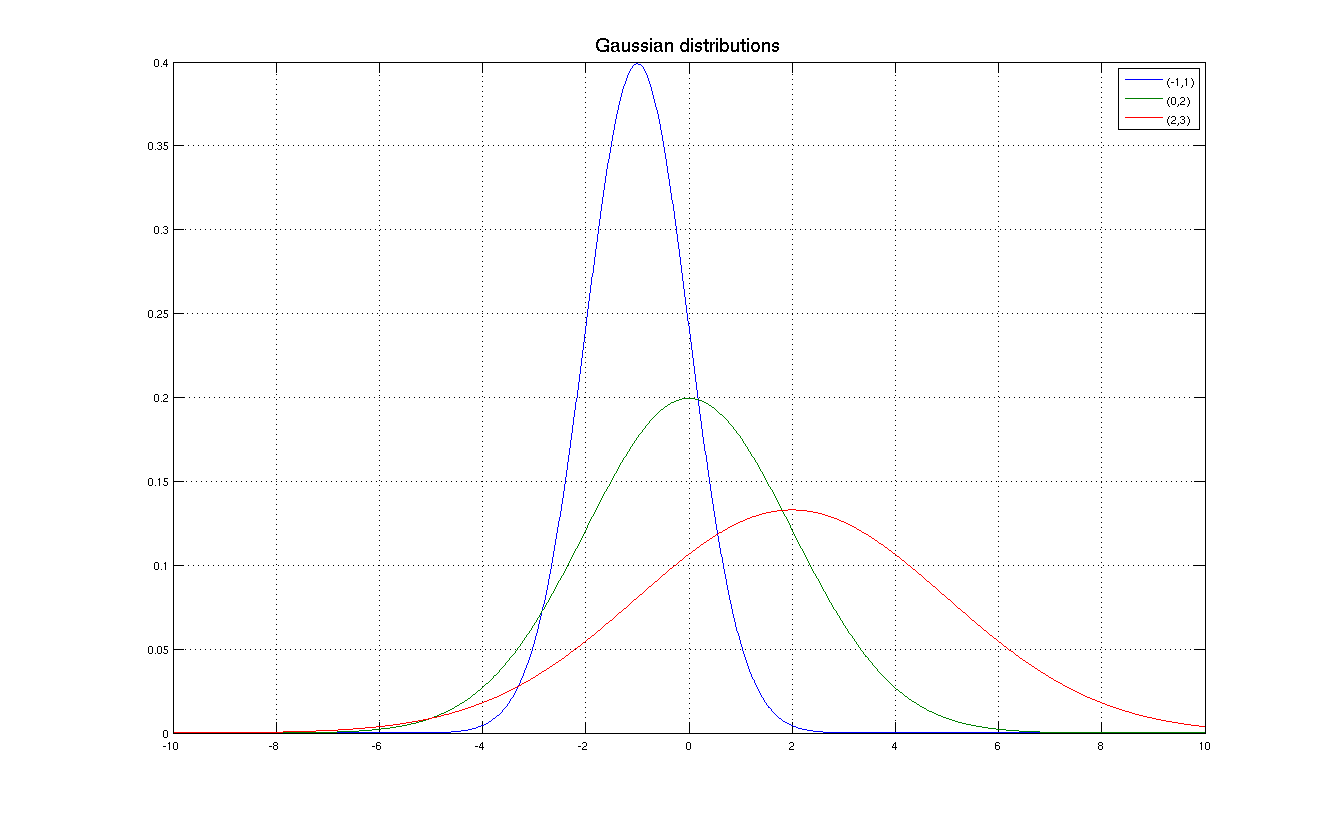
\includegraphics[width=\textwidth]{img/unigauss}
	\caption{Gaussian distributions plotted with different values for
          (\mu, \sigma). \label{fig:I.2.1}}
\end{figure}

\section*{I.2.2}
Source code is available in \texttt{multigauss.m} and \texttt{multigauss\_run.m}.
Plot can be seen in Figure~\ref{fig:I.2.2}.
\begin{figure}[h!]
	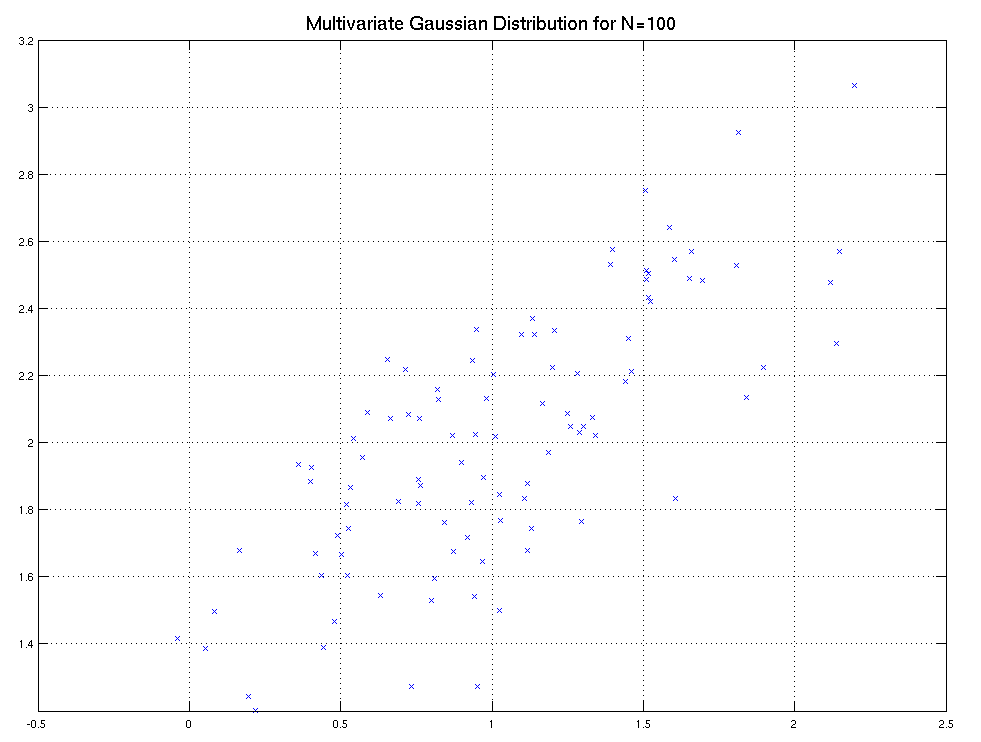
\includegraphics[width=\textwidth]{img/multigauss}
	\caption{100 points drawn from a 2-dimensional Multivariate gaussian
          distribution. \label{fig:I.2.2}}
\end{figure}

\section*{I.2.3}
The \textit{l}2 norm of $x$ is
\begin{align*}
	mean  &= \begin{pmatrix}1 & 2\end{pmatrix}^T \\
	\mu   &= \begin{pmatrix}1.0006 & 1.9834\end{pmatrix}^T \\
	||x|| &= l2(mean - \mu) = 0.0366
\end{align*}
where $l2()$ is a function that calculates the \textit{Euclidean norm} or \textit{l}2
norm of the vector $mean - \mu$.

Figure~\ref{fig:I.2.3} plots the points drawn along with a red circle for the
calculated mean and a green circle for $\mu$. There is a difference between the
two because the mean is calculated based on the generated data drawn from the
multivariate gaussian distribution at random. If we had a number of points
approaching infinite, the difference would approach $\overline{0}$.

\begin{figure}[h!]
	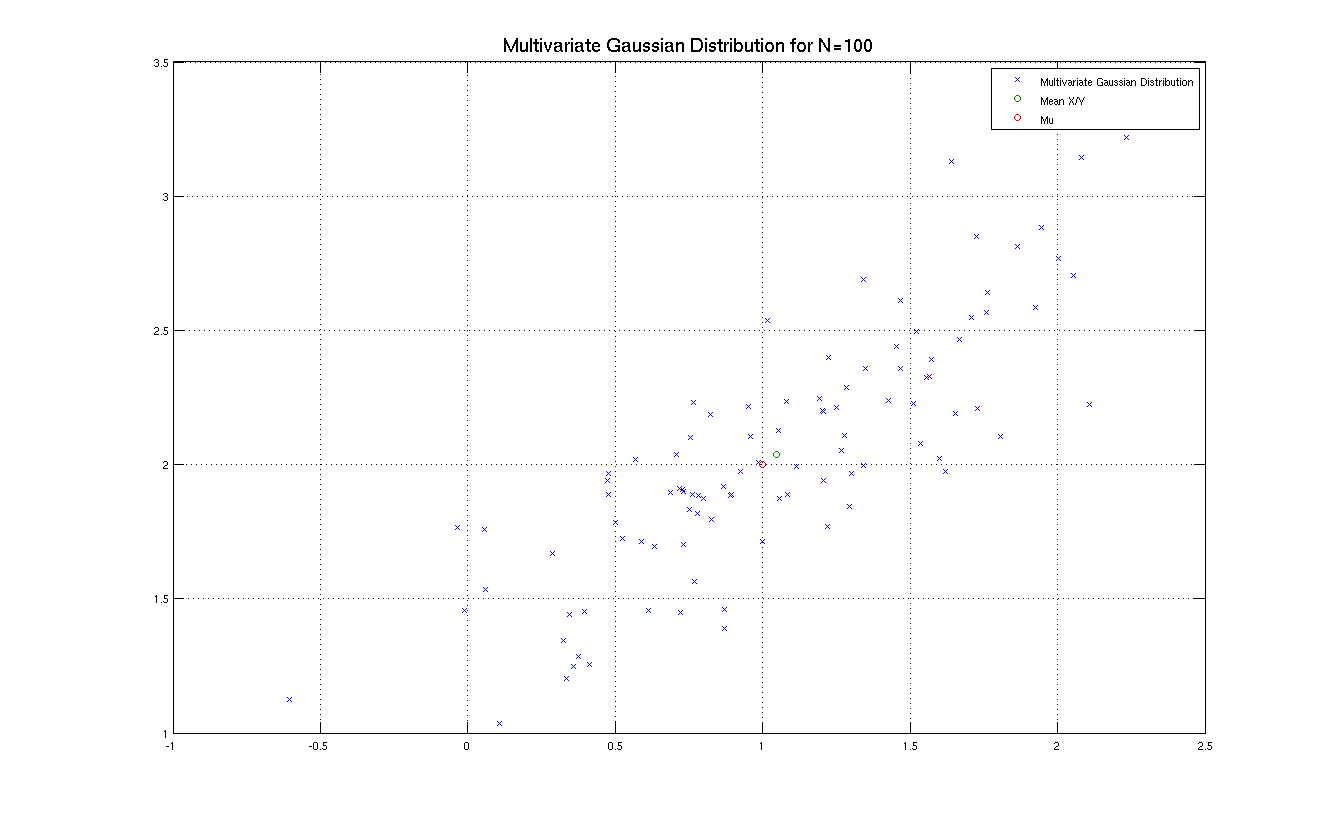
\includegraphics[width=\textwidth]{img/multigaussmeanxy}
	\caption{100 points drawn from a 2-dimensional Multivariate gaussian
          distribution, plotted with the mean of the points and of $\mu$.
        \label{fig:I.2.3}}
\end{figure}

\FloatBarrier
\section*{I.2.4}
The covariance matrix is full rank 2 and thus has two eigenvectors and
eigenvalues. Each eigenvector represents a principal component (or linearly
uncorrelated variable), and each eigenvalue a scalar representing the variance.
Intuitively, the eigenvectors form a scaled and translated coordinate system
centered at the mean of the multivariate Gaussian distribution ($\mu$). If an
eigenvalue is 0, the dimensionality is reduced by one. The larger of the two
eigenvector/value pairs represents the direction where the ellipsis is widest.

The covariance matrix we calculated can be found in
Eq~\ref{eq:cov}. Figure~\ref{fig:I.2.4.1} shows a plot of the Multivariate
gaussian distribution, plotted with the mean, $\mu$ and the two eigenvectors
centered in the distribution $\mu$. Figure~\ref{fig:I.2.4.1.rot} shows a plot of
the 3 rotated distributions along with the distribution rotated to match the
largest eigenvector along the x-axis. The angle needed for this was $-37.2564^o$
in our case.

\begin{align}
	\Sigma_{ML} &= \frac{1}{N} \sum_{n=1}^N (x_n - \mu_{ML}) (x_n - \mu_{ML})^T \notag \\
	&= \begin{pmatrix}
		0.3239 & 0.2093 \\
		0.2093 & 0.2080
	\end{pmatrix} \label{eq:cov}
\end{align}

\begin{figure}[h!]
	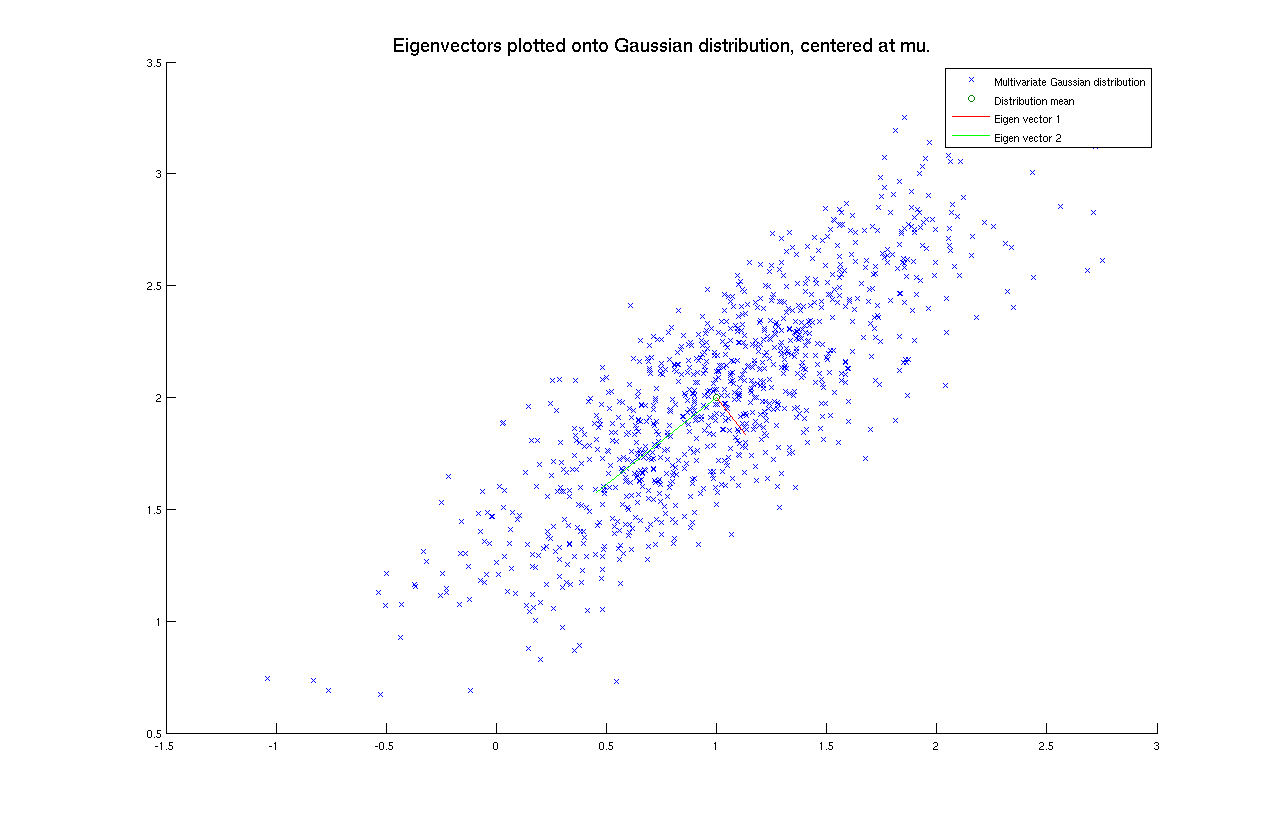
\includegraphics[width=\textwidth]{img/multigausseigen}
	\caption{100 points drawn from a 2-dimensional Multivariate gaussian
          distribution, plotted with the mean of the distribution, the value of
          $\mu$ and the two eigenvectors centered in the distribution
          $\mu$. \label{fig:I.2.4.1}}
\end{figure}

\begin{figure}[h!]
	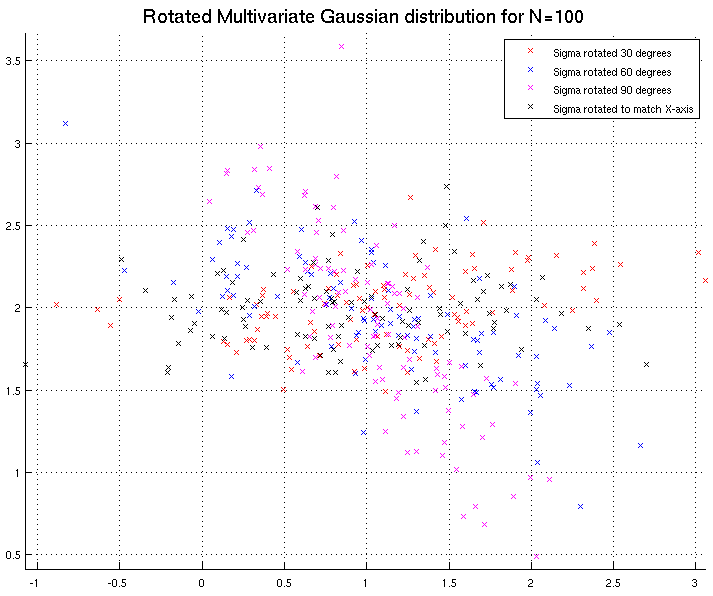
\includegraphics[width=\textwidth]{img/multigaussrotate}
	\caption{100 points drawn from a 2-dimensional Multivariate gaussian
          distribution, rotated at 30, 60 and 90 degrees and lastly also aligned
          along the x-axis, all distributions in their own
          color. \label{fig:I.2.4.1.rot}}
\end{figure}

\section*{I.3}
Given:
\begin{align*}
	\mu = \begin{pmatrix}
		\mu_a \\
		\mu_b \\
		\mu_c
	\end{pmatrix} \quad
	x = \begin{pmatrix}
		x_a \\
		x_b \\
		x_c
	\end{pmatrix} \quad
	\Sigma = \begin{bmatrix}
		\Sigma_{aa} & \Sigma_{ab} & \Sigma_{ac} \\
		\Sigma_{ba} & \Sigma_{bb} & \Sigma_{bc} \\
		\Sigma_{ca} & \Sigma_{cb} & \Sigma_{cc}
	\end{bmatrix}
\end{align*}
We wish to discover an expression for the conditional distribution $p(x_a|x_b)$
in which $x_c$ has been marginalized out. We first find an expression for
$p(x_a|x_b)$ and then marginalize out $x_c$.

We partition $\mu$, $x$ and $\Sigma$ as follows:
\begin{align*}
	\mu &= \begin{pmatrix}
		\mu_d \\
		\mu_c
	\end{pmatrix}, \text{where } \mu_d = \begin{pmatrix}\mu_a \\ \mu_b \end{pmatrix} \\
	\overline{x} &= \begin{pmatrix}
		x_d \\
		x_c
	\end{pmatrix}, \text{where } x_d = \begin{pmatrix}x_a \\ x_b \end{pmatrix} \\
	\Sigma &= \begin{bmatrix}
		\Sigma_{aad} & \Sigma_{abd} \\
		\Sigma_{bad} & \Sigma_{bbd} \\
	\end{bmatrix} \\
	\text{where } \Sigma_{aad} &= \begin{bmatrix}
		\Sigma_{aa} & \Sigma_{ab} \\
		\Sigma_{ba} & \Sigma_{bb}
	\end{bmatrix} \\
	\text{and } \Sigma_{abd} &= \begin{bmatrix}
		\Sigma_{ac} \\ \Sigma_{bc}
	\end{bmatrix} \\
	\text{and } \Sigma_{bad} &= \begin{bmatrix}
		\Sigma_{ca} & \Sigma_{cb}
	\end{bmatrix} \\
	\text{and } \Sigma_{bbd} &= \begin{bmatrix} \Sigma_{cc} \end{bmatrix}
\end{align*}

We also partition the precision matrix
(inverse of the covariance matrix), as:
\begin{align}
	\Lambda &\equiv \Sigma^{-1} = \begin{bmatrix}
		\Lambda_{aa} & \Lambda_{ab} \\
		\Lambda_{ba} & \Lambda_{bb}
	\end{bmatrix}
\end{align}
\textit{Note: This recasts our problem to be to find a conditional distribution
$p(x_d|x_c)$ and then to marginalize $x_c$ out}

A conditional distribution can be evaluated from the joint distribution $p(x) =
p(x_d, x_c)$ by fixing $x_c$ and normalizing. We know from \cite{book} that if a
joint distribution $p(x_d, x_c)$ is Gaussian, then the conditional distribution
$p(x_d|x_c)$ is also Gaussian.

We wish to find $p(x_d | x_c)$, by considering the quadratic form in the
exponent of the Gaussian distribution:

\begin{align}
	& -\frac{1}{2} (x - \mu)^T \Sigma^{-1}(x - \mu) = \label{eq:2.70}\\
	& -\frac{1}{2} (x_d - \mu_d)^T \Lambda_{aa} (x_d - \mu_d) \notag \\
	& -\frac{1}{2} (x_d - \mu_d)^T \Lambda_{ab} (x_c - \mu_c) \notag \\
	& -\frac{1}{2} (x_c - \mu_c)^T \Lambda_{ba} (x_d - \mu_d) \notag \\
	& -\frac{1}{2} (x_c - \mu_c)^T \Lambda_{bb} (x_c - \mu_c) \notag
\end{align}

A Gaussian distribution is completely characterized by its mean and covariance,
so we must find expressions for the mean and covariance of $p(x_d|x_c)$, by
completing the square. We denote the mean and covariance of this distribution by
$\mu_{d|c}$ and $\Sigma_{d|c}$ respectively. By considering the functional
dependence of Eq~\ref{eq:2.70} on $x_d$ in which $x_c$ is regarded as a
constant, we pick out all terms that are second order in $x_d$:
\begin{align}
	-\frac{1}{2} x_d^T \Lambda_{aa} x_d
\end{align}
From which we have that $\Sigma_{d|c} = \Lambda_{aa}^{-1}$. The terms in
Eq~\ref{eq:2.70} which are linear in $x_d$ are $x_d^T \left \{ \Lambda_{aa}
\mu_d - \Lambda_{a}(x_c - \mu_c) \right \}$, making use of the fact that
$\Lambda_{ba}^T = \Lambda_{ab}$ (See \cite[p.85]{book}). The coefficient of
$x_d$ in this expression is equal to $\Sigma_{d|c}^{-1} \mu_{d|c}$ and so:

\begin{align}
	\mu_{d|c} &= \Sigma_{d|c} \left\{ \Lambda_{aa} \mu_{d} - \Lambda_{ab}(x_c - \mu_c) \right\} \notag \\
		  &= \mu_d - \Lambda_{aa}^{-1} \Lambda_{ab}(x_c - \mu_c) \label{eq:2.75}
\end{align}

Making use of the \textit{Schur complement} of a matrix\cite[p.87]{book}, we
have that:
\begin{align*}
	\Lambda_{aa} &= (\Sigma_{aa} - \Sigma_{ab} \Sigma_{bb}^{-1} \Sigma_{ba})^{-1} \\
	\Lambda_{ab} &= -(\Sigma_{aa} - \Sigma_{ab} \Sigma_{bb}^{-1} \Sigma_{ba})^{-1} \Sigma_{ab} \Sigma_{bb}^{-1}
\end{align*}

From these we now have the following for the mean and covariance of $p(x_d|x_c)$:
\begin{align}
	\mu_{d|c} &= \mu_d + \Sigma_{ab} \Sigma_{bb}^{-1} (x_c - \mu_c) \\
	\Sigma_{d|c} &= \Sigma_{aa} - \Sigma_{ab} \Sigma_{bb}^{-1} \Sigma_{ba}
\end{align}

We must now find the margina distribution given by
\begin{align*}
	p(x_d) = \int p(x_d, x_c) \ dx_c
\end{align*}

We complete the square to integrate out $x_c$. The terms involving $x_c$ are:
\begin{align*}
	-\frac{1}{2} x_c^T \Lambda_{bb} x_c + x_c^T m = \\
	-\frac{1}{2} (x_c - \Lambda_{bb}^{-1} m)^T \Lambda_{bb} (x_c - \Lambda_{bb}^{-1} m)
	+\frac{1}{2} m^T \Lambda_{bb}^{-1} m
\end{align*}
Where $m = \Lambda_{bb} \mu_c - \Lambda_{ba} (x_d - \mu_d)$. This is again a
standard quadratic form, and we note that the integration becomes an integral
over an unnormalized Gaussian, whereby the result is the reciprocal of the
normalization coefficient\cite[p. 88]{book}. The normalization coefficient
depends only on the determinant of the covariance matrix, so we can integrate
out $x_c$ and the only term remaining that depends on $x_d$ is $m$. Combined
with the remaining terms from Eq~\ref{eq:2.70} that depend on $x_d$ we have:
\begin{align*}
	\frac{1}{2} & [ \Lambda_{bb} \mu_c - \Lambda_{ba} (x_d - \mu_d)]^T \Lambda_{bb}^{-1} [\Lambda_{bb} \mu_c - \Lambda_{ba}(x_d - \mu_d)] \\
	-\frac{1}{2} & x_d^T \Lambda_{aa} x_d + x_d^T (\Lambda_{aa} \mu_d + \Lambda_{ab} \mu_c) + \text{const} \\
	= -\frac{1}{2} & x_d^T(\Lambda_{aa} - \Lambda_{ab} \Lambda_{bb}^{-1} \Lambda_{ba}) x_d \\
	+ & x_d^T (\Lambda_{aa} - \Lambda_{ab} \Lambda_{bb}^{-1} \Lambda_{ba})^{-1} \mu_d + \text{const}
\end{align*}
Where `const' is quantities independent of $x_d$. The covariance and mean of the
marginal distribution $p(x_d)$ are thus
\begin{align*}
	\Sigma_d &= (\Lambda_{aa} - \Lambda_{ab} \Lambda_{bb}^{-1} \Lambda_{ba})^{-1} \\
	\mu_d &= \Sigma_d (\Lambda_{aa} - \Lambda_{ab} \Lambda_{bb}^{-1} \Lambda_{ba}) \mu_d = \mu_d \quad \text{(See \cite[p.89,Eq~2.89]{book})}
\end{align*}
Making use of the \textit{Schur complement} again we have that $(\Lambda_{aa} -
\Lambda_{ab} \Lambda_{bb}^{-1} \Lambda_{ba})^{-1} = \Sigma_{aa}$. Finally we
have that $\mathbb{E}[x_d] = \mu_d$ and $\text{cov}[x_d] =
\Sigma_{aa}$. Intuitively, to obtain the marginal distribution over a subset of
multivariate normal random variables, we drop the variables we want to
marginalize out from the mean and covariance.

\pagebreak
\section{I.4}
\subsection{I.4.1}
The result of our KNN implementation for different k-values and datasets is
shown in Table \ref{tab:knn-res}. The file that generates these results is
\texttt{kNN\_run.m}, it will setup the experiment and do the classifying using
the funktion defined in \texttt{kNN.m}.
\begin{table}
\center
\begin{tabular}{|l|l|l|}
\hline
Description          & $K$-value & Accuracy in \% \\\hline
Run on training data & 1         & $100  \%$ \\
Run on test data     & 1         & $81.5 \%$ \\
Run on training data & 3         & $86.0 \%$ \\
Run on test data     & 3         & $81.5 \%$ \\
Run on training data & 5         & $83.0 \%$ \\
Run on test data     & 5         & $68.4 \%$ \\\hline
\end{tabular}
\caption{The results from I.4}
\label{tab:knn-res}
\end{table}

With $K=1$ and running against the training set, the accuracy is 100\% since any
entry will be matched against itself, and only itself. We also see a general
loss of accuracy as $K$ increases, this is because the point gets matched up
against a larger and larger part of the total points, meaning it will become
more likely to be classified as the type of point there is occuring most times
in the training set.


\subsection{I.4.2}
The program run for this experiment is \texttt{fivefold\_val.m}, it will use aux
functions from \texttt{kNN.m}, \texttt{shuffleSplit.m} and
\texttt{bucketJoiner.m}. We first split the training data using the
\texttt{shuffleSplit} function, it creates a cell-table that contains a
specified number of ``subsets'' that collectively is the entire training set,
but where the indices of the data is shuffled. We then assemble these parts into
2 sets, one that is 1/5 of the data, which will be used as a testing set, and
one with 4/5 of the data, which is the training set.  using five different
partitions of the data (with the above method) we used the \texttt{kNN} function
from the previous subsection to benchmark the different $K$ values with 5
``different training sets''.

During this test, a $K$ value of $5$ gets the best accuracy, around 80\%, but
when run against the actual training set, which have not been used or considered
in the above process, the accuracy drops to $68,4\%$. This is the same accuracy
we got from $K=5$ in the previous section.

\subsection{I.4.3}
The program used for this experiment is \texttt{fivefold\_val\_normalized.m}
which is similar to the above experiment, except it also utilizes
\texttt{scale.m} to normalize the test data.  The $(\text{mean},\text{var})$ of
the training data is: $(3.0288,7.8218)$, the test data after the normalization
have the values $(0.1545,1.0000)$. The most optimal $K$ value is still 5, but
the accuracy have increased to $71,05\%$ when using the normalized test set.
